Een cluster bestaat uit vele onderdelen die gezamenlijk ervoor zorgen dat een cluster beheersbaar blijft. Laten we beginnen met de opbouw van het systeem. Een container\index{container} is de kleinst mogelijk eenheid. Een container bevat een applicatie met zijn afhankelijkheden. Containers worden opgestart in pods, een pod\index{pod} is \'e\'en of meer containers die samen moeten worden opgestart, gedraaid en afgesloten. Ze zijn onderling van elkaar afhankelijk. Een container kan bijvoorbeeld een webserver bevatten die bestanden van een opslagsysteem serveert en een tweede container bevat een applicatie die ervoor zorgt dat de bestanden gesynchroniseert blijven met de master. De ene container kan niet draaien zonder de ander. Het heeft geen zin om een webserver te draaien met verouderde data en data synchroniseren zonder dat ze gebruikt worden is ook zinloos. Deze twee containers moeten dus tegelijk aanwezig zijn en dus komen ze in een pod.

Pods, draaien op een container runtime\index{container!runtime}. Zegmaar een hypervisor voor containers/pods. En een container runtime draait uiteindelijk op een operating system. Tussen de container runtime en het OS zit een interface die we de CRI\index{CRI} (Container Runtime Interface)\index{container runtime interface} noemen.

\begin{figure}[H]
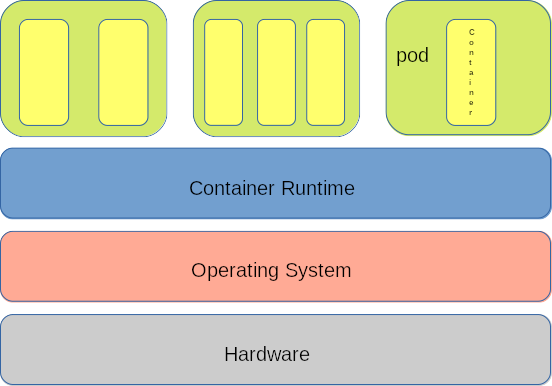
\includegraphics[width=0.99\linewidth]{container_runtime}
	\caption{Container runtime}
	\label{ref:container_runtime}
\end{figure}
